\section{未命名节}

\subsection{无隐状态的神经网络}

\subsection{8.4.1 无隐状态的神经网络}

\subsection{8.4.1 无隐状态的神经网络}
\begin{center}
\Large \textcolor{blue}{从简单开始:没有记忆的网络}
\end{center}


\paragraph{尝试1:直接用MLP}
\textbf{想法:}用多层感知机直接建模语言模型

$$P(x_t \mid x_{t-1}, x_{t-2}, \ldots, x_{t-\tau})$$

\begin{center}
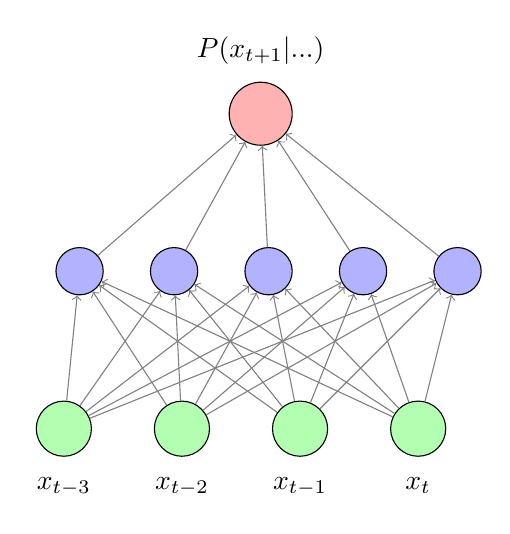
\begin{tikzpicture}[scale=1.0]
% 输入层
\foreach \i in {1,2,3,4} {
    \node[circle,draw,fill=green!30,minimum size=0.7cm] (i\i) at (\i*1.5,0) {};
}
\node[below] at (1.5,-0.5) {$x_{t-3}$};
\node[below] at (3,-0.5) {$x_{t-2}$};
\node[below] at (4.5,-0.5) {$x_{t-1}$};
\node[below] at (6,-0.5) {$x_t$};

% 隐藏层
\foreach \i in {1,2,3,4,5} {
    \node[circle,draw,fill=blue!30,minimum size=0.6cm] (h\i) at (\i*1.2+0.5,2) {};
}

% 输出层
\node[circle,draw,fill=red!30,minimum size=0.8cm] (o) at (4,4) {};
\node[above] at (4,4.5) {$P(x_{t+1}|...)$};

% 连接
\foreach \i in {1,2,3,4} {
    \foreach \j in {1,2,3,4,5} {
        \draw[->,thin,gray] (i\i) -- (h\j);
    }
}
\foreach \i in {1,2,3,4,5} {
    \draw[->,thin,gray] (h\i) -- (o);
}

\end{tikzpicture}
\end{center}

\textbf{问题:}
\begin{itemize}
    \item 输入维度固定为 $\tau$
    \item 参数数量随 $\tau$ 增长
    \item 无法处理变长序列
\end{itemize}


\paragraph{MLP语言模型的局限}
\begin{center}
\begin{tikzpicture}[scale=1.0]
% 窗口大小问题
\node[draw,fill=red!20,text width=10cm] at (5,3.5) {
\textbf{问题1:窗口大小固定}
\begin{itemize}
    \item $\tau=4$:只能看4个词
    \item 长期依赖无法捕捉
    \item ``I grew up in France... I speak fluent \_\_\_''
\end{itemize}
};

% 参数爆炸
\node[draw,fill=orange!20,text width=10cm] at (5,1.8) {
\textbf{问题2:参数数量}
\begin{itemize}
    \item 输入层:$\tau \times d_{embed}$
    \item 词表大:$V=10000$,$\tau=100$ $\Rightarrow$ 百万级参数
\end{itemize}
};

% 无法共享
\node[draw,fill=yellow!20,text width=10cm] at (5,0.3) {
\textbf{问题3:无法参数共享}
\begin{itemize}
    \item 处理位置1和位置2的``the''用不同参数
\end{itemize}
};

\end{tikzpicture}
\end{center}


\paragraph{需要一个"记忆装置"}
\textbf{核心思想:}引入\textbf{隐状态}作为记忆

\begin{center}
\begin{tikzpicture}[scale=1.1]
% 对比
\node[text width=4.5cm,align=center] at (2,3.5) {
\textbf{MLP:无记忆}
};

\node[text width=4.5cm,align=center] at (8,3.5) {
\textbf{RNN:有记忆}
};

% MLP
\foreach \i in {1,2,3} {
    \node[circle,draw,fill=blue!20,minimum size=0.5cm] (m\i) at (\i*0.8,2) {};
}
\node[circle,draw,fill=green!30,minimum size=0.6cm] at (1.6,1) {输出};
\draw[->,thick] (m1) -- (1.6,1.3);
\draw[->,thick] (m2) -- (1.6,1.3);
\draw[->,thick] (m3) -- (1.6,1.3);
\node[below,font=\tiny,text width=3cm,align=center] at (1.6,0.5) {每次重新开始};

% RNN
\node[circle,draw,fill=red!20,minimum size=0.6cm] (h1) at (6.5,2) {$h_1$};
\node[circle,draw,fill=red!20,minimum size=0.6cm] (h2) at (7.5,2) {$h_2$};
\node[circle,draw,fill=red!20,minimum size=0.6cm] (h3) at (8.5,2) {$h_3$};
\node[circle,draw,fill=red!20,minimum size=0.6cm] (h4) at (9.5,2) {$h_4$};

\draw[->,thick,blue] (h1) -- (h2);
\draw[->,thick,blue] (h2) -- (h3);
\draw[->,thick,blue] (h3) -- (h4);
\node[below,font=\tiny,text width=3cm,align=center] at (8,0.5) {隐状态记住历史};

\end{tikzpicture}
\end{center}

\begin{theorem}[关键]
隐状态 $h_t$ 总结了到时刻 $t$ 为止的所有历史信息
\end{theorem}



\subsection{有隐状态的循环神经网络}

\subsection{8.4.2 有隐状态的循环神经网络}

\subsection{8.4.2 有隐状态的循环神经网络}
\begin{center}
\Large \textcolor{blue}{RNN的核心:循环连接}
\end{center}


\paragraph{RNN的基本结构}
\textbf{核心思想:}隐状态在时间步之间传递

\begin{definition}[数学定义]
\begin{align*}
\mathbf{H}_t &= \phi(\mathbf{X}_t \mathbf{W}_{xh} + \mathbf{H}_{t-1}\mathbf{W}_{hh} + \mathbf{b}_h) \\
\mathbf{O}_t &= \mathbf{H}_t \mathbf{W}_{hq} + \mathbf{b}_q
\end{align*}
\end{definition}

\textbf{符号说明:}
\begin{itemize}
    \item $\mathbf{X}_t \in \mathbb{R}^{n \times d}$:时间步 $t$ 的输入($n$ 个样本)
    \item $\mathbf{H}_t \in \mathbb{R}^{n \times h}$:隐状态($h$ 是隐藏单元数)
    \item $\mathbf{O}_t \in \mathbb{R}^{n \times q}$:输出($q$ 是输出维度)
    \item $\mathbf{W}_{xh} \in \mathbb{R}^{d \times h}$:输入到隐藏的权重
    \item $\mathbf{W}_{hh} \in \mathbb{R}^{h \times h}$:隐藏到隐藏的权重
    \item $\mathbf{W}_{hq} \in \mathbb{R}^{h \times q}$:隐藏到输出的权重
    \item $\phi$:激活函数(通常是 $\tanh$)
\end{itemize}


\paragraph{RNN的计算图}
\begin{center}
\begin{tikzpicture}[scale=1.2]
% 隐藏层
\foreach \i in {1,2,3,4} {
    \node[circle,draw,fill=red!20,minimum size=1cm] (h\i) at (\i*2.5,2) {$\mathbf{H}_{\i}$};
}

% 输入层
\foreach \i in {1,2,3,4} {
    \node[circle,draw,fill=green!20,minimum size=0.8cm] (x\i) at (\i*2.5,0) {$\mathbf{X}_{\i}$};
}

% 输出层
\foreach \i in {1,2,3,4} {
    \node[circle,draw,fill=blue!20,minimum size=0.8cm] (o\i) at (\i*2.5,4) {$\mathbf{O}_{\i}$};
}

% 连接
\foreach \i in {1,2,3,4} {
    \draw[->,thick] (x\i) -- (h\i) node[midway,right,font=\tiny] {$\mathbf{W}_{xh}$};
    \draw[->,thick] (h\i) -- (o\i) node[midway,right,font=\tiny] {$\mathbf{W}_{hq}$};
}

% 循环连接
\foreach \i in {1,2,3} {
    \pgfmathtruncatemacro{\next}{\i+1}
    \draw[->,very thick,blue] (h\i) -- (h\next) node[midway,above,font=\tiny] {$\mathbf{W}_{hh}$};
}

% 标注
\node[below] at (5,-0.7) {\textbf{关键:}相同的权重在所有时间步共享!};

\end{tikzpicture}
\end{center}


\paragraph{RNN的展开视图}
\textbf{将循环展开成前馈网络:}

\begin{center}
\begin{tikzpicture}[scale=0.9]
% 折叠视图
\node[draw,fill=yellow!20,text width=3cm,align=center] at (0,2) {
\textbf{折叠视图}\\
循环结构
};

\node[circle,draw,fill=red!20,minimum size=1cm] (h) at (0,0) {$\mathbf{H}$};
\node[circle,draw,fill=green!20] (x) at (-1.5,-1.5) {$\mathbf{X}$};
\node[circle,draw,fill=blue!20] (o) at (1.5,-1.5) {$\mathbf{O}$};

\draw[->,thick] (x) -- (h);
\draw[->,thick] (h) -- (o);
\draw[->,thick,blue] (h) to[out=135,in=45,looseness=8] (h);

% 箭头
\draw[->,ultra thick] (2,0) -- (4,0) node[midway,above] {展开};

% 展开视图
\node[draw,fill=yellow!20,text width=3cm,align=center] at (9,2) {
\textbf{展开视图}\\
前馈网络
};

\foreach \i in {1,2,3} {
    \node[circle,draw,fill=red!20,minimum size=0.8cm] (H\i) at (5+\i*1.5,0) {$\mathbf{H}_{\i}$};
    \node[circle,draw,fill=green!20,minimum size=0.6cm] (X\i) at (5+\i*1.5,-1.5) {$\mathbf{X}_{\i}$};
    \node[circle,draw,fill=blue!20,minimum size=0.6cm] (O\i) at (5+\i*1.5,1.5) {$\mathbf{O}_{\i}$};
    
    \draw[->,thick] (X\i) -- (H\i);
    \draw[->,thick] (H\i) -- (O\i);
}

\draw[->,thick,blue] (H1) -- (H2);
\draw[->,thick,blue] (H2) -- (H3);

\end{tikzpicture}
\end{center}

\begin{theorem}[关键特点]
\begin{itemize}
    \item 展开后是一个很深的网络(深度=序列长度)
    \item 所有时间步\textbf{共享相同的参数} $\mathbf{W}_{xh}, \mathbf{W}_{hh}, \mathbf{W}_{hq}$
\end{itemize}
\end{theorem}


\paragraph{RNN的参数共享}
\textbf{为什么参数共享?}

\begin{center}
\begin{tikzpicture}[scale=1.0]
% 时间步1
\node[draw,fill=blue!20,minimum size=1cm] (h1) at (0,2) {$\mathbf{H}_1$};
\node[draw,fill=green!20] (x1) at (0,0.5) {$\mathbf{X}_1$};
\draw[->,thick] (x1) -- (h1) node[midway,right,font=\tiny,red] {$\mathbf{W}_{xh}$};

% 时间步2
\node[draw,fill=blue!20,minimum size=1cm] (h2) at (3,2) {$\mathbf{H}_2$};
\node[draw,fill=green!20] (x2) at (3,0.5) {$\mathbf{X}_2$};
\draw[->,thick] (x2) -- (h2) node[midway,right,font=\tiny,red] {$\mathbf{W}_{xh}$};
\draw[->,thick] (h1) -- (h2) node[midway,above,font=\tiny,red] {$\mathbf{W}_{hh}$};

% 时间步3
\node[draw,fill=blue!20,minimum size=1cm] (h3) at (6,2) {$\mathbf{H}_3$};
\node[draw,fill=green!20] (x3) at (6,0.5) {$\mathbf{X}_3$};
\draw[->,thick] (x3) -- (h3) node[midway,right,font=\tiny,red] {$\mathbf{W}_{xh}$};
\draw[->,thick] (h2) -- (h3) node[midway,above,font=\tiny,red] {$\mathbf{W}_{hh}$};

% 标注
\node[below,text width=8cm,align=center,font=\small] at (3,-0.5) {
\textcolor{red}{相同的权重} $\Rightarrow$ 处理``the''用同样的变换
};

\end{tikzpicture}
\end{center}

\textbf{优点:}
\begin{itemize}
    \item $\checkmark$ 参数数量与序列长度无关
    \item $\checkmark$ 可以处理任意长度的序列
    \item $\checkmark$ 学到的模式可以迁移到序列的任何位置
\end{itemize}


\paragraph{RNN的前向传播过程}
\textbf{逐步计算:}

\begin{enumerate}
    \item \textbf{初始化:}$\mathbf{H}_0 = \mathbf{0}$(或学习得到)
    
    \item \textbf{时间步1:}
    \begin{align*}
    \mathbf{H}_1 &= \tanh(\mathbf{X}_1 \mathbf{W}_{xh} + \mathbf{H}_0 \mathbf{W}_{hh} + \mathbf{b}_h) \\
    \mathbf{O}_1 &= \mathbf{H}_1 \mathbf{W}_{hq} + \mathbf{b}_q
    \end{align*}
    
    \item \textbf{时间步2:}
    \begin{align*}
    \mathbf{H}_2 &= \tanh(\mathbf{X}_2 \mathbf{W}_{xh} + \mathbf{H}_1 \mathbf{W}_{hh} + \mathbf{b}_h) \\
    \mathbf{O}_2 &= \mathbf{H}_2 \mathbf{W}_{hq} + \mathbf{b}_q
    \end{align*}
    
    \item \textbf{...重复...}
\end{enumerate}

\begin{theorem}[关键]
每一步都依赖前一步的隐状态 $\mathbf{H}_{t-1}$
\end{theorem}


\paragraph{激活函数的选择}
\textbf{为什么用 $\tanh$?}

\begin{center}
\begin{tikzpicture}[scale=1.0]
% 坐标轴
\draw[->,thick] (-3,0) -- (3,0) node[right] {$x$};
\draw[->,thick] (0,-1.5) -- (0,1.5) node[above] {$y$};

% tanh曲线
\draw[blue,thick,domain=-2.5:2.5,samples=100] plot (\x,{tanh(\x)});
\node[blue,right] at (2,1) {$\tanh(x)$};

% 标注
\draw[dashed] (-3,1) -- (3,1);
\draw[dashed] (-3,-1) -- (3,-1);
\node[left] at (0,1) {1};
\node[left] at (0,-1) {-1};

% 特点
\node[below,text width=6cm,align=center] at (0,-2.2) {
\small 输出范围:$[-1, 1]$ | 平滑 | 零中心
};

\end{tikzpicture}
\end{center}



\textbf{优点:}
\begin{itemize}
    \item 输出有界
    \item 零中心(mean=0)
    \item 梯度更稳定
\end{itemize}


\textbf{也可以用:}
\begin{itemize}
    \item ReLU:计算快
    \item sigmoid:$[0,1]$输出
    \item 但 $\tanh$ 最常用
\end{itemize}



\paragraph{RNN前向传播代码}
\begin{lstlisting}
def rnn_forward(inputs, state, params):
    """ inputs: sequence,shape (batch_size, vocab_size) state: (batch_size, num_hiddens) params: [W_xh, W_hh, b_h, W_hq, b_q] """
    W_xh, W_hh, b_h, W_hq, b_q = params
    outputs = []
    H = state
    
    for X in inputs:
        H = torch.tanh(torch.mm(X, W_xh) + torch.mm(H, W_hh) + b_h)
        # Output
        Y = torch.mm(H, W_hq) + b_q
        outputs.append(Y)
    
    return torch.cat(outputs, dim=0), H
\end{lstlisting}

\begin{definition}[关键点]
\begin{itemize}
    \item 循环遍历每个时间步
    \item 隐状态 $H$ 不断更新
    \item 返回所有输出和最终隐状态
\end{itemize}
\end{definition}


\paragraph{隐状态的继续输出}
\textbf{维度分析}

\begin{definition}[重要:理解各个张量的形状]
\begin{center}
\begin{tabular}{|l|c|l|}
\hline
\textbf{变量} & \textbf{形状} & \textbf{说明} \\
\hline
$\mathbf{X}_t$ & $(n, d)$ & 批量大小$n$,输入维度$d$ \\
\hline
$\mathbf{H}_t$ & $(n, h)$ & 批量大小$n$,隐藏单元数$h$ \\
\hline
$\mathbf{W}_{xh}$ & $(d, h)$ & 输入到隐藏 \\
\hline
$\mathbf{W}_{hh}$ & $(h, h)$ & 隐藏到隐藏 \\
\hline
$\mathbf{W}_{hq}$ & $(h, q)$ & 隐藏到输出 \\
\hline
$\mathbf{b}_h$ & $(h,)$ & 隐藏层偏置 \\
\hline
$\mathbf{b}_q$ & $(q,)$ & 输出层偏置 \\
\hline
\end{tabular}
\end{center}

\begin{example}[示例]
批量大小 $n=32$,输入维度 $d=256$,隐藏单元 $h=128$,输出维度 $q=100$
\end{example}
\end{definition}



\subsection{基于循环神经网络的字符级语言模型}

\subsection{8.4.3 基于循环神经网络的字符级语言模型}

\subsection{8.4.3 基于循环神经网络的字符级语言模型}
\textbf{目标:}用RNN构建字符级语言模型

\begin{center}
\Large \textcolor{blue}{实现一个能生成文本的RNN模型}
\end{center}


\paragraph{字符级语言模型}
\begin{center}
\begin{tikzpicture}[scale=1.0]
% MLP
\node[draw,fill=blue!20] at (0,2) {\textbf{任务:}预测下一个字符};

% 输入序列
\node[font=\small] at (-1.5,3) {\textbf{MLP(窗口$\tau=100$)}};
\foreach \i/\c in {0/t,1/h,2/e,3/{ },4/t,5/i,6/m,7/e} {
    \node[draw,fill=green!20,minimum size=0.6cm] at (\i*0.8,2) {\tiny\c};
}

% RNN处理
\node[font=\small] at (-1,1.5) {\textbf{RNN}};
\node[draw,fill=green!20,text width=4.5cm] at (6,2.5) {
\textbf{RNN}\\
$\mathbf{W}_{xh}$:$d \times h$\\
$\mathbf{W}_{hh}$:$h \times h$\\
$\mathbf{W}_{hq}$:$h \times V$\\
\textcolor{green!60!black}{\textbf{总计:固定!}}
};

% 箭头
\foreach \i in {0,...,6} {
    \pgfmathtruncatemacro{\next}{\i+1}
    \draw[->,thick,blue] (\i*0.8,2) -- (\next*0.8,2);
}

% 输出预测
\node[font=\small] at (-1,0.5) {预测:};
\foreach \i/\c in {1/h,2/e,3/{ },4/t,5/i,6/m,7/e} {
    \node[draw,fill=red!20,minimum size=0.6cm] at (\i*0.8,0) {\c};
}

% 连接
\foreach \i in {0,...,6} {
    \draw[->,thick] (\i*0.8,1.8) -- (\i*0.8,0.2);
}
\node[left] at (5,2.3) {序列越长};
\node[below] at (6,0) {\textcolor{green!60!black}{参数不变}};

\end{tikzpicture}
\end{center}

\begin{definition}[RNN的优势]
参数共享使得RNN可以高效处理任意长度的序列
\end{definition}

\paragraph{字符级语言模型}
\begin{center}
\Large \textcolor{blue}{给定``the''预测``h'',给定``th''预测``e''...}
\end{center}

\begin{theorem}[关键思想]
每个时间步都进行预测,使用\textbf{teacher forcing}训练
\end{theorem}


\paragraph{One-Hot编码}
\textbf{字符 $\rightarrow$ 向量}

\begin{center}
\begin{tabular}{|c|c|}
\hline
\textbf{字符} & \textbf{One-Hot向量} \\
\hline
'a' & $[1,0,0,0,0]$ \\
\hline
'b' & $[0,1,0,0,0]$ \\
\hline
'c' & $[0,0,1,0,0]$ \\
\hline
'd' & $[0,0,0,1,0]$ \\
\hline
'e' & $[0,0,0,0,1]$ \\
\hline
\end{tabular}
\end{center}

\begin{definition}[特点]
\begin{itemize}
\item 向量维度 = 词汇表大小
\item 每个向量只有一个1,其余为0
\item 稀疏表示,计算效率低
\end{itemize}
\end{definition}



\subsection{困惑度}


\subsection{8.4.4 困惑度}

\subsection{8.4.4 困惑度(Perplexity)}
\textbf{定义:}评估语言模型性能的指标

$$\textbf{PPL} = \exp\left(-\frac{1}{N}\sum_{t=1}^{N}\log p(x_t|x_{<t})\right)$$



\textbf{好的模型:}
\begin{itemize}
\item 高概率预测下一个词
\item 低困惑度
\item PPL = $\exp(0.25) \approx$ 1.3
\end{itemize}


\textbf{差的模型:}
\begin{itemize}
\item 低概率预测下一个词
\item 高困惑度
\item PPL = $\exp(2.3) \approx$ 10
\end{itemize}


\begin{theorem}[直观理解]
困惑度 = 模型在预测时的"平均选择数量"
\end{theorem}


